\chapter{Moment法}
Moment法とはVu Van Hungらが開発した,熱膨張,自由エネルギーなどを見積もることができる計算手法である.
特徴としては,
\begin{itemize}
 \item 原子間の相互作用エネルギーの高次微分を利用することによって,非調和効果を取り込んだ計算が可能.
 \item 熱膨張を計算したのち,その格子の長さから自由エネルギーの計算を行うため体積変化を考慮した計算が可能.
 \item 経験的なペアポテンシャルでの計算を前提としている.
 \item 系に$a$の外力が働いているときの系の平均変位$\left<u_i\right>_a$という値を利用する.
\end{itemize}
などが挙げられる.本章では,そんなMoment法の計算手法,また,経験的なペアポテンシャルを利用したfcc構造での計算手法について記述する.

\section{外力が無い場合の変位$y_0$の導出}
Moment法では熱膨張の計算をする際,原子の変位から系の外力なしの場合の変位を求める関数$y_0$を利用する.
本節ではその関数の導出を行う.

$N$個の原子が線形結合していると考えると,相互作用エネルギーは
\begin{eqnarray}
\label{eq:moment1}
U=N\sum_{i}\varphi_{i0}(|a_i+u_i|)
\end{eqnarray}
と書くことができる.ここで$\varphi_{i0}$は0番目と$i$番目の原子間のポテンシャルエネルギー,$a_i$は$i$番目の原子の平衡位置,$u_i$は$i$番目の原子の平衡位置からの変位である.
$\varphi_{i0}(|a_i+u_i|)$を変位$u_i$についてテイラー展開を行い4次の項まで取ると次式ができる.
\begin{eqnarray}
\label{eq:moment2}
\varphi_{i0}(|a_i+u_i|)=\varphi_{i0}(|a_i|)+
\frac{1}{2}\left( \frac{\delta^2\varphi_{i0}}{\delta u_i^2} \right) u_i^2+
\frac{1}{6}\left( \frac{\delta^3\varphi_{i0}}{\delta u_i^3} \right) u_i^3+
\frac{1}{24}\left( \frac{\delta^4\varphi_{i0}}{\delta u_i^4} \right) u_i^4
\end{eqnarray}
この式はポテンシャルエネルギーなので変位$u_i$で微分すると,
\begin{eqnarray}
\label{eq:moment3}
\left( \frac{\delta^2\varphi_{i0}}{\delta u_i^2} \right) u_i+
\frac{1}{2}\left( \frac{\delta^3\varphi_{i0}}{\delta u_i^3} \right) u_i^2+
\frac{1}{6}\left( \frac{\delta^4\varphi_{i0}}{\delta u_i^4} \right) u_i^3
\end{eqnarray}
となり,0番目の原子に作用する力が得られる.
ここで,$a$を系に働いている外力,$\left<u_i\right>_a$を外力$a$が働いているときの$u_i$の平均変位とし,系が平衡状態であるという条件を加えると以下の等式を作ることができる.
\begin{eqnarray}
\label{eq:moment4}
\sum_i\left( \frac{\delta^2\varphi_{i0}}{\delta u_i^2} \right) \left<u_i\right>_a+
\frac{1}{2}\sum_i\left( \frac{\delta^3\varphi_{i0}}{\delta u_i^3} \right) \left<u_i^2\right>_a+
\frac{1}{6}\sum_i\left( \frac{\delta^4\varphi_{i0}}{\delta u_i^4} \right) \left<u_i^3\right>_a- a =0
\end{eqnarray}
この式は,左辺第三項までが,外力$a$が働いている際の平均変位による力を表しており,外力$a$との差が0という等式により,系の平衡状態を表している.この平均変位$\left<u_i\right>_a$を利用するのがMoment法の大きな特徴である.
Vu Van Hungらによると,$\left<u_i\right>_a$,$\left<u_i^2\right>_a$,$\left<u_i^3\right>_a$は次のようになる\cite[p.514]{jindo2}.
\begin{eqnarray}
\label{eq:moment5}
&\left<u_i\right>_a& \equiv y\\
\label{eq:moment6}
&\left<u_i^2\right>_a& = \left<u_i\right>_a^2 + \theta \frac{\delta\left<u_i\right>_a}{\delta a} + \frac{\theta}{k}(x \coth x-1)\\
\label{eq:moment7}
&\left<u_i^3\right>_a& = \left<u_i\right>_a^3 + 3 \theta \left<u_i\right>_a \frac{\delta\left<u_i\right>_a}{\delta a} 
+\theta^2 \frac{\delta^2\left<u_i\right>_a}{\delta a^2} 
+ \frac{\theta}{k}(x \coth x-1) \left<u_i\right>_a
\end{eqnarray}
\begin{eqnarray}
\label{eq:moment8}
k \equiv 
\sum_i\left( \frac{\delta^2\varphi_{i0}}{\delta u_i^2}\right)
\equiv
m\omega^2, \;
x=\frac{\hbar\omega}{2\theta},\;
\theta = k_{\rm{B}}T,\;
\gamma\equiv\frac{1}{6}\sum_i\left( \frac{\delta^4\varphi_{i0}}{\delta u_i^4} \right)
\end{eqnarray}
$m$は質量,$\omega$は角振動数,$\hbar$はプランク定数を$2\pi$で割ったもの,$k_{\rm{B}}$はボルツマン定数,$T$は温度である.
また,$k$は式\ref{eq:moment4}の左辺第一項に含まれている2次微分成分,$\gamma$は左辺第3項に含まれている4次微分成分である.
式(\ref{eq:moment4})に式(\ref{eq:moment5}),(\ref{eq:moment6}),(\ref{eq:moment7})を代入すると次式が得られる.また,線形結合のため$\left( \frac{\delta^3\varphi_{i0}}{\delta u_i^3} \right)$は0となり消えている.
\begin{eqnarray}
\label{eq:moment9}
\gamma\theta^2 \frac{\delta^2y}{\delta a^2}
+3\gamma\theta y \frac{\delta y}{\delta a}
+\gamma y^3 + ky
+ \frac{\gamma \theta}{k}(x\coth x-1)-a=0
\end{eqnarray}
式(\ref{eq:moment9})には,$\frac{\delta^2y}{\delta a^2}$と$\frac{\delta y}{\delta a}$が含まれている.
これを解くために
\begin{eqnarray}
\label{eq:moment10}
y=y_0+A_1a+A_2a^2
\end{eqnarray}
このように$y$を$a$の関数で表すことにする.$A_1$,$A_2$は任意の値である.$y_0$は外力なしの平衡位置からの変位であり,本節で求めることになる関数である.$y$は$\left<u_i\right>_a$であり,熱膨張の計算において計算者が入力とする平衡位置からの変位である.$a$を含んだ右辺第2,3項は外力による平衡位置からの変位を表している.
これらにより左辺$y$は外力なしの変位と外力による変位の和であり,外力を考慮した変位であるとわかる.
式(\ref{eq:moment9})と式(\ref{eq:moment10})を利用して$A_2$が消えるように式変形を行うと次式が得られる.
\begin{eqnarray}
\label{eq:moment11}
3\gamma y_0^4+\Big[3k+6\gamma \theta A_1+\frac{3\gamma \theta}{k}(x\coth x-1) \Big] y_0^2\nonumber \\ 
-\Big[k\theta A_1-\theta + \frac{\gamma \theta^2}{k}(x \coth x -1)A_1+3\gamma \theta^2 A_1^2 \Big]=0
\end{eqnarray}
ここからは近似を用いて$A_1$の導出を行う.まずは,式(\ref{eq:moment9})を,$ky-a=0$という簡単な形にする.それにより,$A_1=\frac{1}{k}$と置くことができ,式(\ref{eq:moment11})に代入すると,
\begin{eqnarray}
\label{eq:moment12}
3\gamma y_0^4+3k\left[1+ \frac{\gamma \theta}{k^2}(x\coth x+1)\right]y_0^2
  -\frac{2\gamma \theta^2}{k^2}\left(
    1+\frac{x \coth x}{2}
   \right)=0
\end{eqnarray}
となる.ここで,$y_0^2$は$\frac{k}{\gamma}$に対して十分大きいため,
\begin{eqnarray}
\label{eq:moment13}
y_0^2 \approx \frac{2\gamma\theta^2}{3k^3}\left(1+\frac{x \coth x}{2}\right)
\end{eqnarray}
と近似することができる.この式(\ref{eq:moment13})を式(\ref{eq:moment11})に代入すると
\begin{eqnarray}
\label{eq:moment14}
A_1\approx\frac{1}{k}\left[ 1+ \frac{2\gamma^2\theta^2}{k^4}\left(1+\frac{x\coth x}{2}(x \coth x + 1)\right)\right]
\end{eqnarray}
となり,精度の高い$A_1$得ることができる.$A_1$の導出が完了したので,式(\ref{eq:moment14})と式(\ref{eq:moment11})を利用することで,
\begin{eqnarray}
\label{eq:moment15}
y_0^2&\approx &\frac{2\gamma\theta^2}{3k^3}A,\\
A&=&a_1
+\frac{\gamma^2 \theta^2}{k^4}a_2
+\frac{\gamma^3 \theta^3}{k^6}a_3
+\frac{\gamma^4 \theta^4}{k^8}a_4,\nonumber \\
a_1&=&\frac{x \coth x}{2}+1,\nonumber \\
a_2&=&\frac{1}{2}x^3 \coth x^3
+\frac {23}{6} x^2 \coth x^2
+\frac {47}{6}x \coth x
+\frac{13}{3},\nonumber \\
a_3&=&-\left(
\frac{1}{2}x^4 \coth x^4
+\frac{16}{3}x^3 \coth x^3
+\frac{50}{3}x^2 \coth x^2
+\frac{121}{6}x \coth x
+\frac{25}{3}
\right),\nonumber \\
a_4&=&
\frac{1}{2}x^5 \coth x^5
+7x^4 \coth x^4
+\frac{250}{9}x^3 \coth x^3
+46x^2 \coth x^2
+\frac{199}{6}x \coth x
+\frac{77}{9}.\nonumber
\end{eqnarray}
$y_0$を導出することができる.
\subsection{$y_0$の不一致}
この$y_0$の値はVu Van Hungらの$y_0$と比べると,$a_4$の値が一致していない.
Vu Van Hungらの$a_4$は
\begin{eqnarray}
\label{eq:vua4}
a_4&=&
\frac{1}{2}x^5 \coth x^5
+\frac{22}{3}x^4 \coth x^4
+\frac{83}{3}x^3 \coth x^3
+\frac{169}{3}x^2 \coth x^2
+\frac{93}{2}x \coth x
+\frac{43}{3}\nonumber
\end{eqnarray}
である.$y_0$は$k$, $\gamma$, 温度$T$の関数であり,$T$を100K, 900Kとしたときの$a_4$の違いによる$y_0$の値を図\ref{fig:vuvana4}に示す.横軸に最近接原子間距離,縦軸が$y_0$の値であり,計算にはCuのペアポテンシャルの$k$,$\gamma$を使用した.100Kでは値の差はないが900Kでは原子間距離が伸びるに連れて若干の差が出ていることがわかる.Moment法は高温域で大きく熱膨張する傾向が見られるため,今回は導出した式(\ref{eq:moment15})を使うことにする.
\begin{figure}[htbp]
 \begin{minipage}[b]{0.5\linewidth}
  \centering
  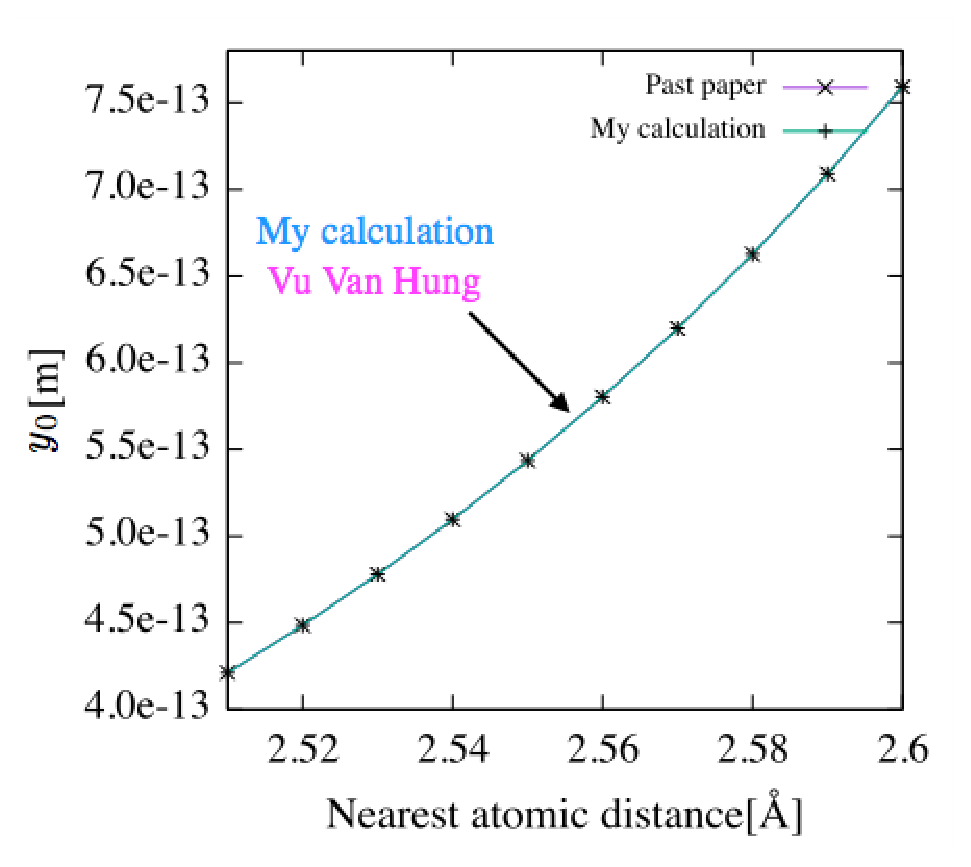
\includegraphics[keepaspectratio, scale=0.42]
  {../image/a4_1_label.eps}
  \subcaption{$T$=100K}\label{a41}
 \end{minipage}
 \begin{minipage}[b]{0.5\linewidth}
  \centering
  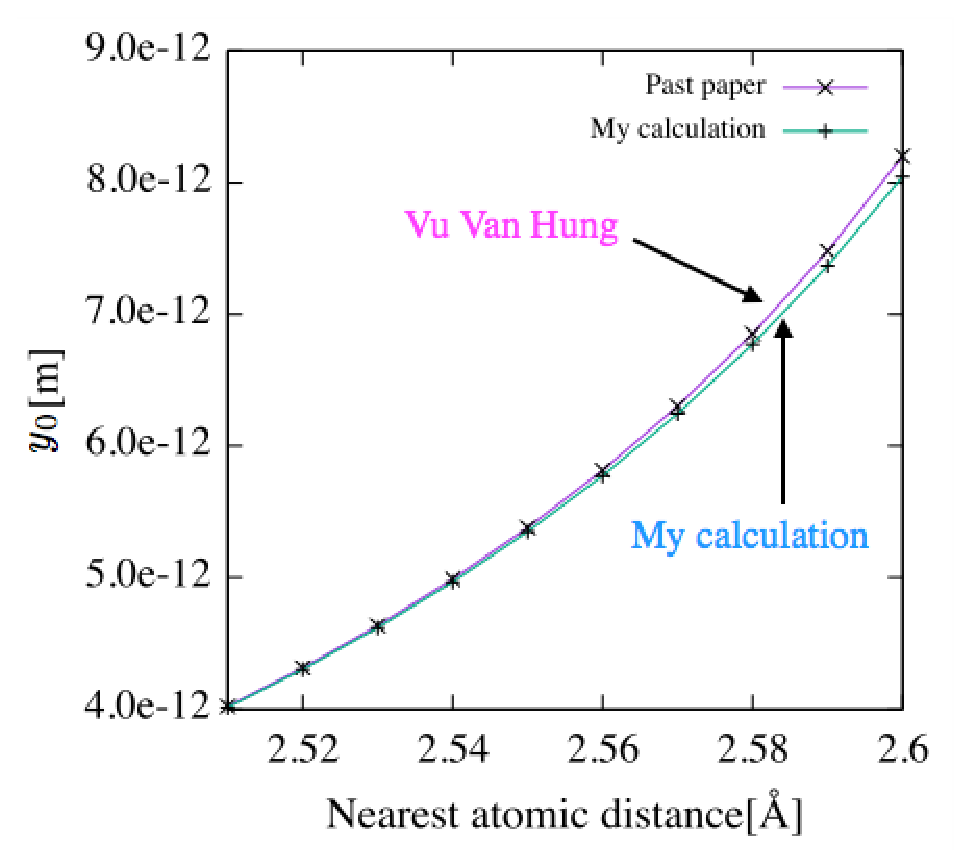
\includegraphics[keepaspectratio, scale=0.42]
  {../image/a4_2_label.eps}
  \subcaption{$T$=900K}\label{a42}
 \end{minipage}
 \caption{導出した$a_4$と参考文献の$a_4$による$y_0$の比較.}\label{fig:vuvana4}
\end{figure}
\section{熱膨張の計算}
\label{sec:heatexpantion} 
前節で外力が無い場合の変位$y_0$の導出をおこなった.本節ではそれを利用した熱膨張の計算について記述する.
まずは$y_0$の導出の際に使用した式(\ref{eq:moment10})に注目する.
左辺$y$は計算者の設定する平衡原子間距離からの変位である.
右辺第一項$y_0$は外力がない場合の変位であり,右辺の残りの項は外力による変位を表している.
ここで$y=y_0$となる場合,右辺第2, 3項が0となる.すなわち,外力による変位が0であり,その時の$y$は外力の影響の無い,熱膨張のみを考慮した変位となる.
$y$と$y_0$の関係を図\ref{fig:yy0}に示す.$y$と平衡原子間距離を足し合わせた原子間距離から,ポテンシャルの2次微分成分$k$,4次微分成分$\gamma$の値がわかる.その後,$k$,$\gamma$の値から$y_0$が算出される.

\begin{figure}[htbp]
 \begin{center}
  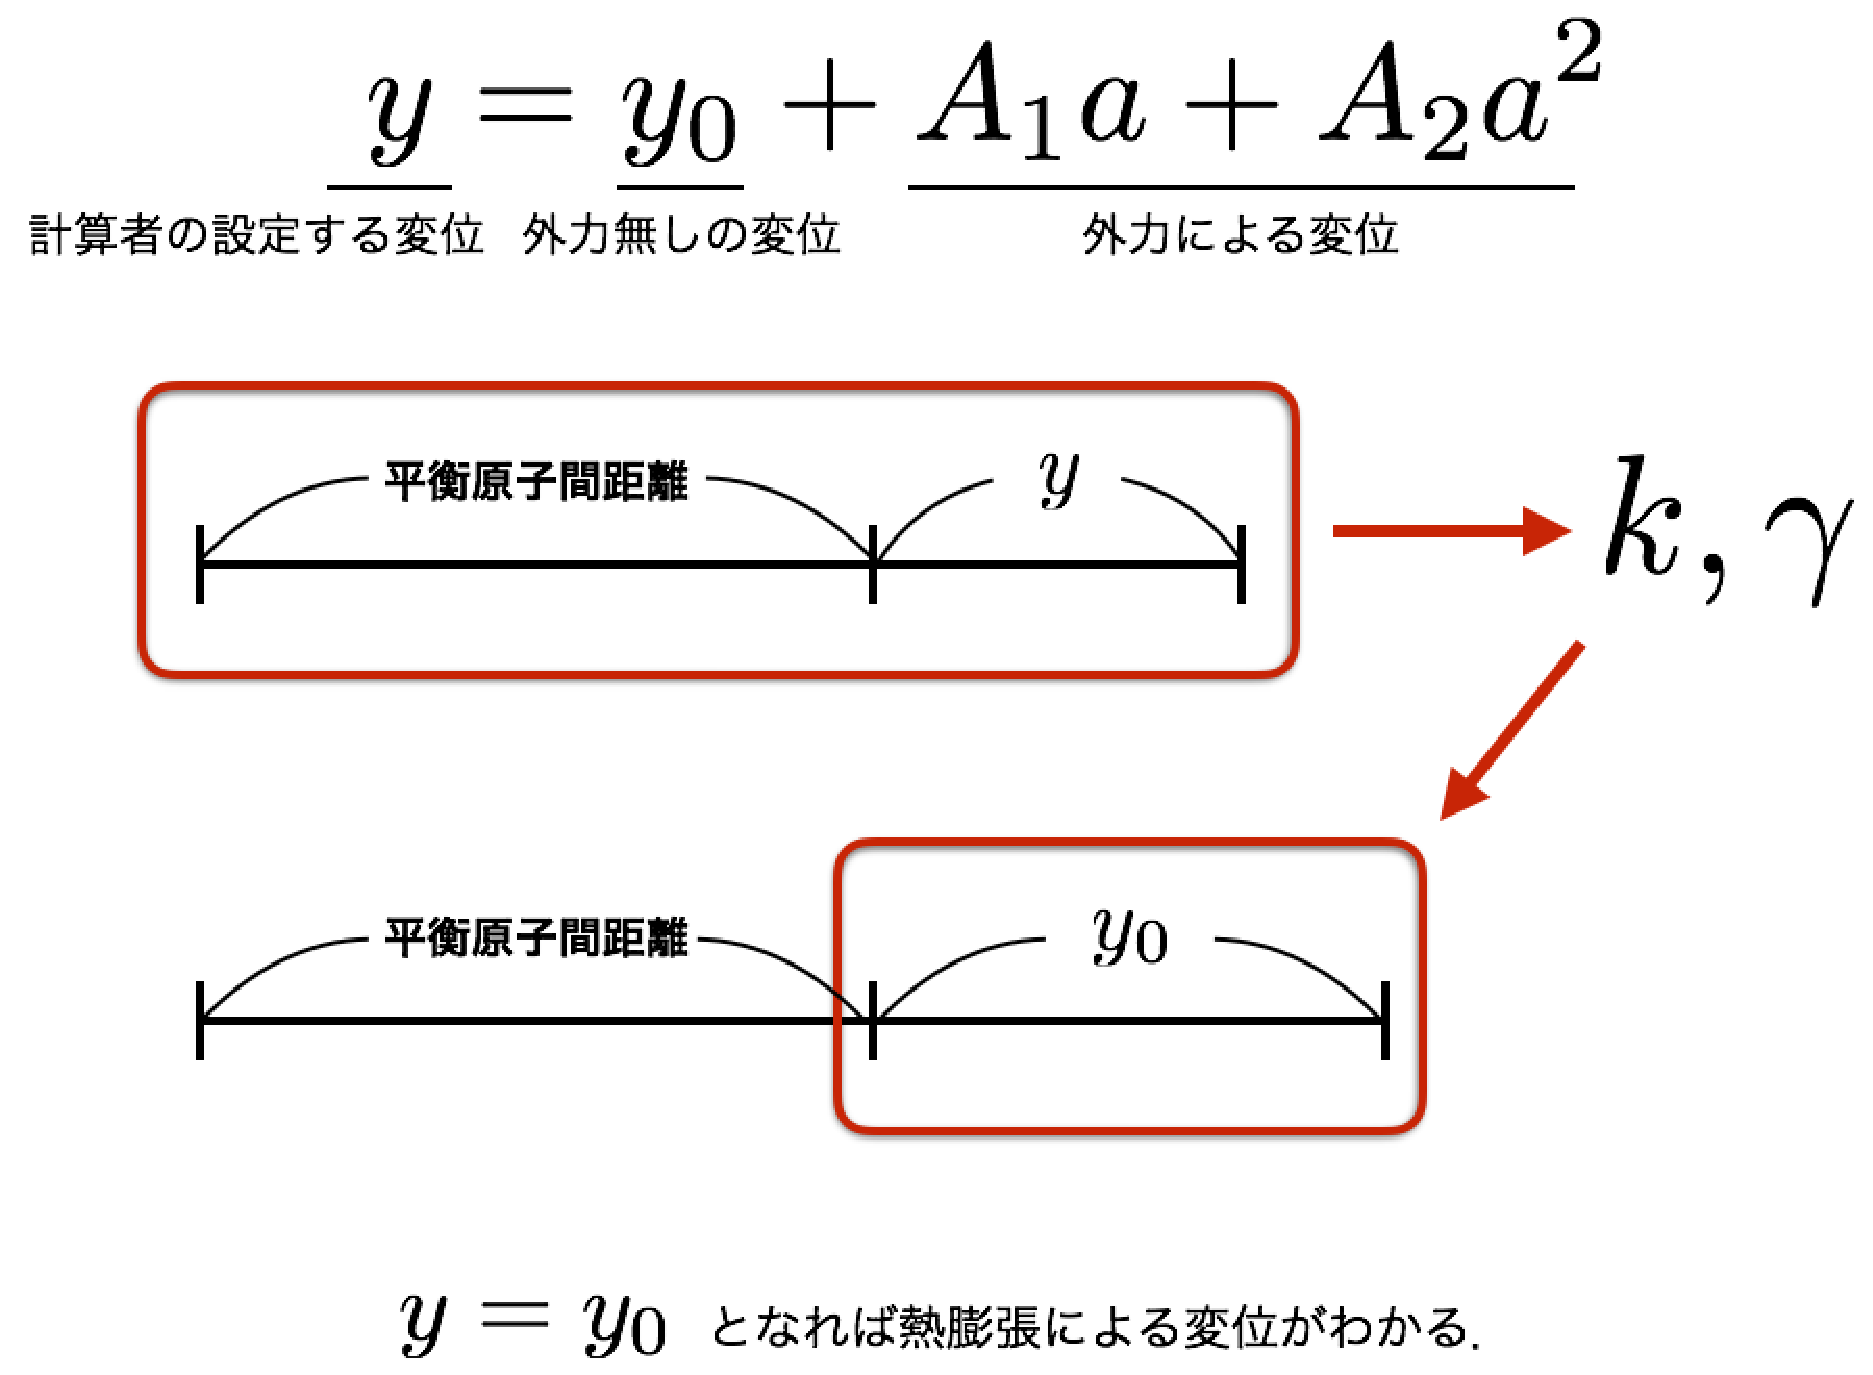
\includegraphics[width=130mm]{../image/fig1.eps}
 \end{center}
 \caption{$y$と$y_0$の関係図.}
 \label{fig:yy0}
\end{figure}


\section{線形結合の自由エネルギー計算}
熱膨張が求まった際,系は外力がない状態である.
その状態のでの原子の変位から$k$, $\gamma$の値を取り出し,自由エネルギーを算出することができる.
Vu Van Hungらによれば,線形結合の自由エネルギー$\psi$は次式となる\cite[p.515]{jindo2}.

\begin{eqnarray}
\label{eq:moment16}
\psi \approx U_0+\psi_0-\frac{N\gamma\theta^2}{6k^2}\left(1+\frac{x \coth x}{2}\right)
-\frac{N\gamma^2\theta^3}{4k^4}\left(1+\frac{x \coth x}{2}\right)(x \coth x + 1)
\end{eqnarray}
\begin{eqnarray}
\label{eq:moment17}
U_0\equiv N\sum_i\varphi_{i0}(|a_i|)
\end{eqnarray}
\begin{eqnarray}
\label{eq:moment18}
\varphi_0 = N\theta[x+\log{(1-e^{-2x})}]
\end{eqnarray}
$U_0$は原子間相互作用によるポテンシャルエネルギーであり,内部エネルギーとも呼ぶ.$\psi_0$は調和振動による自由エネルギーである.式(\ref{eq:moment16})の第3項からは非調和振動による自由エネルギーである.
また$N$は原子数であり,単純に$\psi$全体を$N$倍している.
\section{fcc構造での計算}
\label{sec:fcc}
ここまでは線形結合での計算を示した.実際の格子構造で計算するためには,経験的ペアポテンシャルで格子構造を再現し計算を行わなければならない.本節ではペアポテンシャルを利用したfcc構造での計算手法について記述する.

\subsection{$k$, $\gamma$の導出}
Moment法はポテンシャルの2次微分である$k$,4次微分を6で割った$\gamma$に依存する.
fcc構造では原子配置を考慮すると,式(\ref{eq:moment8})の$k$, $\gamma$の値が次式に置き換わる.
\begin{eqnarray}
\label{eq:moment19}
k \equiv 
\sum_i\left( \frac{\delta^2\varphi_{i0}}{\delta u_{iX}^2}\right),\,
\gamma\equiv\frac{1}{6}\sum_i\left[\left( \frac{\delta^4\varphi_{i0}}{\delta u_{iX}^4} \right)
+6\left( \frac{\delta^4\varphi_{i0}}{\delta u_{iX}^2\delta u_{iY}^2} \right)
\right]
\end{eqnarray}
ここで$X$,$Y$はそれぞれ原子間距離の$x$,$y$成分を表しており,$\frac{\delta^2\varphi_{i0}}{\delta u_{iX}^2}$,$\frac{\delta^4\varphi_{i0}}{\delta u_{iX}^4}$はそれぞれポテンシャルの$x$成分の2次,4次微分を表している.
また,$\frac{\delta^4\varphi_{i0}}{\delta u_{iX}^2\delta u_{iY}^2}$は,ポテンシャルの$x$成分で2次微分,$y$成分で2次微分を表している.
以下に$k$の導出方法を示す.

原子間距離$r$を$x$,$y$,$z$成分で表すと,
\begin{eqnarray}
\label{eq:moment20}
r=\sqrt{x^2+y^2+z^2}
\end{eqnarray}
である.これを考慮してポテンシャル$\varphi(r)$を$x$で2次微分すると次式が得られる.
\begin{eqnarray}
\label{eq:moment21}
\frac{\delta^2\varphi(r)}{\delta x^2}=
\frac{\delta^2 \varphi(r)}{\delta r^2} \frac{x^2}{x^2+y^2+z^2}
-\frac{\delta \varphi(r)}{\delta r} \frac{x^2}{(x^2+y^2+z^2)^{3/2}}
+\frac{\delta \varphi(r)}{\delta r} \frac{1}{\sqrt{x^2+y^2+z^2}}
\end{eqnarray}
これで$\frac{\delta^2\varphi_{i0}}{\delta u_{iX}^2}$の導出は完了であり,ここからは$\sum_i$の計算を行う.
この式にfcc構造の第1近接原子12個,第2近接原子6個の相対的な座標をそれぞれ代入し和を取るとfcc構造の$k$を得ることができる.
\begin{eqnarray}
\label{eq:momentk}
k=
4\frac{\delta^2 \varphi(a_1)}{\delta r^2}
+\frac{8}{a_1}\frac{\delta \varphi(a_1)}{\delta r}
+2\frac{\delta^2 \varphi(a_2)}{\delta r^2}
+\frac{4}{a_2}\frac{\delta \varphi(a_2)}{\delta r}
\end{eqnarray}
ここで,$a_1$は第1近接原子,$a_2$は第2近接原子である.同様の操作で$\sum_i\left(\frac{\delta^4\varphi_{i0}}{\delta u_{iX}^4}\right)$と
$\sum_i\left(\frac{\delta^4\varphi_{i0}}{\delta u_{iX}^2\delta u_{iY}^2}\right)$を計算すると,

\begin{eqnarray}
\label{eq:moment22}
\sum_i \left( \frac{\delta^4\varphi_{i0}}{\delta u_{iX}^4} \right)=
2\frac{\delta^4 \varphi(a_1)}{\delta r^4}
+\frac{12}{a_1}\frac{\delta^3 \varphi(a_1)}{\delta r^3}
-\frac{6}{a_1^2}\frac{\delta^2 \varphi(a_1)}{\delta r^2}
+\frac{6}{a_1^3}\frac{\delta \varphi(a_1)}{\delta r}\nonumber\\
+2\frac{\delta^4 \varphi(a_2)}{\delta r^4}
+\frac{12}{a_2^2}\frac{\delta^2 \varphi(a_2)}{\delta r^2}
-\frac{12}{a_2^3}\frac{\delta \varphi(a_2)}{\delta r}
\end{eqnarray}

\begin{eqnarray}
\label{eq:moment23}
\sum_i \left(\frac{\delta^4\varphi_{i0}}{\delta u_{iX}^2\delta u_{iY}^2}\right)=
\frac{\delta^4 \varphi(a_1)}{\delta r^4}
+\frac{2}{a_1}\frac{\delta^3 \varphi(a_1)}{\delta r^3}
+\frac{3}{a_1^2}\frac{\delta^2 \varphi(a_1)}{\delta r^2}
-\frac{3}{a_1^3}\frac{\delta \varphi(a_1)}{\delta r}\nonumber\\
+\frac{4}{a_2}\frac{\delta^3 \varphi(a_2)}{\delta r^3}
-\frac{6}{a_2^2}\frac{\delta^2 \varphi(a_2)}{\delta r^2}
+\frac{6}{a_2^3}\frac{\delta \varphi(a_2)}{\delta r}
\end{eqnarray}
となり,$\gamma$は
\begin{eqnarray}
\label{eq:gamma}
\gamma=
\frac{4}{3}\frac{\delta^4 \varphi(a_1)}{\delta r^4}
+\frac{4}{a_1}\frac{\delta^3 \varphi(a_1)}{\delta r^3}
+\frac{2}{a_1^2}\frac{\delta^2 \varphi(a_1)}{\delta r^2}
-\frac{2}{a_1^3}\frac{\delta \varphi(a_1)}{\delta r}\nonumber\\
+\frac{1}{3}\frac{\delta^4 \varphi(a_2)}{\delta r^4}
+\frac{4}{a_2}\frac{\delta^3 \varphi(a_2)}{\delta r^3}
-\frac{4}{a_2^2}\frac{\delta^2 \varphi(a_2)}{\delta r^2}
+\frac{4}{a_2^3}\frac{\delta \varphi(a_2)}{\delta r}
\end{eqnarray}
となる.
これによりfcc構造での$k$, $\gamma$がわかった.
\ref{sec:heatexpantion}節で説明した熱膨張の計算は原子が直線上に並ぶ線形結合を前提としている.
そのため,今回導出した$k$, $\gamma$は$x$方向のみに注目して微分を行うことにより,線形結合の熱膨張の計算に対応できるようにしている.
また,$\gamma$には$y$方向の微分も入っているが,これはペアポテンシャルでfcc構造を再現するために混ぜている.


\subsection{自由エネルギーの計算}
ペアポテンシャルによるfcc構造の自由エネルギーの計算は,線形結合の自由エネルギーとは計算式が異なる.
$\gamma_1$,$\gamma_2$を
\begin{eqnarray}
\label{eq:moment24}
\gamma_1=\frac{1}{24}\sum_i \left( \frac{\delta^4\varphi_{i0}}{\delta u_{iX}^4} \right), 
\gamma_2=\frac{1}{4}\sum_i \left(\frac{\delta^4\varphi_{i0}}{\delta u_{iX}^2\delta u_{iY}^2}\right)
\end{eqnarray}
と定義した時,自由エネルギー$\psi$は次式となる\cite[p.516]{jindo2}.
\begin{align}
\label{eq:moment25}
\psi \approx U_0+\psi_0-
3N\left\{ \frac{\theta^2}{k^2}\left[ \gamma_2x^2 \coth^2 x -\frac{2\gamma_1}{3}\left(1+\frac{x \coth x}{2}\right)\right]\right.\nonumber \\
\left. +\frac{2\theta^3}{k^4}\left[\frac{4}{3}\gamma_2^2 x \coth x \left(1+\frac{x \coth x}{2}\right) \right. \right. \nonumber\\
\left. \left. -2(\gamma_1^2+2\gamma_1\gamma_2)\left(1+\frac{x \coth x}{2}\right)(1+x \coth x)\right]\right\}
\end{align}
\begin{eqnarray}
\label{eq:moment27}
\varphi_0 = 3N\theta[x+\log{(1-e^{-2x})}]
\end{eqnarray}
式(\ref{eq:moment16})と同様に$U_0$は原子間相互作用によるポテンシャルエネルギー,$\psi_0$は調和振動による自由エネルギー,	
第3項からは非調和振動による自由エネルギーとなる.$N$は原子数であり,$3N$を全体にかける形になっている.これは$k$,$\gamma$が$x$方向のみをを考慮にいれており,残りの$y$,$z$方向の値を加えるためである.
